\usetikzlibrary{arrows,calc}

\begin{figure}
\centering
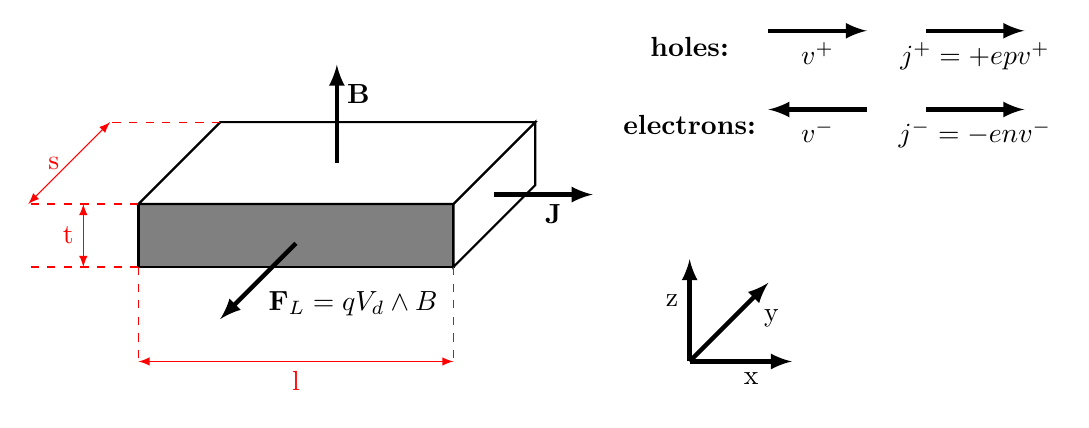
\begin{tikzpicture}
%Grid
%\draw[step=1cm,gray,very thin] (-5,-4) grid (8,4);

% Cube
\pgfmathsetmacro{\cubex}{4};
\pgfmathsetmacro{\cubey}{0.8};
\pgfmathsetmacro{\cubez}{2.7};
% xy rectangle
\draw[fill=gray,thick] (0,0,0) coordinate(o) -- ++(-\cubex,0,0) coordinate(a1) -- ++(0,-\cubey,0) coordinate(a2) -- ++(\cubex,0,0) coordinate(a3) -- cycle;
% yz rectangle
\draw[fill=white,thick] (0,0,0) -- ++(0,0,-\cubez) coordinate(b1) -- ++(0,-\cubey,0) coordinate(b2) -- ++(0,0,\cubez) coordinate(b3) -- cycle;
% xz rectangle
\draw[fill=white,thick] (0,0,0) -- ++(-\cubex,0,0) coordinate(c1)-- ++(0,0,-\cubez) coordinate(c2)-- ++(\cubex,0,0) coordinate(c3)-- cycle;

% Dashed lines
\draw [red,dashed] (a1)--++(-1.4,0) coordinate (s1);
\draw [red,dashed] (a2)--++(-1.4,0);
\draw [red,dashed] (c2)--++(-1.4,0)coordinate (s2);
\draw [red,latex-latex] (s1) -- (s2) node[red,pos=0.5,left]{s};
\draw [red,latex-latex] (-4.7,0) -- (-4.7,-\cubey) node[red,pos=0.5,left]{t};
\draw [red,dashed] (a2)--++(0,-1.2)coordinate(l1);
\draw [red,dashed] (a3)--++(0,-1.2)coordinate(l2);
\draw [red,latex-latex] (l1)--(l2)node[red,pos=0.5,below]{l};

% holes
\node[] at (3,2){\textbf{holes:}};
\draw [ultra thick,-latex] (4,2.2)--++(1.25,0) node[pos = 0.5,below]{$v^{+}$};
\draw [ultra thick,-latex] (6,2.2)--++(1.25,0) node[pos = 0.5,below]{$j^{+}=+e p v^{+}$};

% electrons
\node[] at (3,1){\textbf{electrons:}};
\draw [ultra thick,latex-] (4,1.2)--++(1.25,0) node[pos = 0.5,below]{$v^{-}$};
\draw [ultra thick,-latex] (6,1.2)--++(1.25,0) node[pos = 0.5,below]{$j^{-}=-e n v^{-}$};

% Axis
\pgfmathsetmacro{\length}{1.3};
\coordinate (O) at (3,-2);
\draw [ultra thick,-latex] (O)--++(0,\length)node[pos = 0.6,left]{z};
\draw [ultra thick,-latex] (O)--++(0,0,-\length*2)node[pos = 0.8,below right]{y};
\draw [ultra thick,-latex] (O)--++(\length,0)node[pos = 0.6,below]{x};

%% Labels %%
% F eqn
\draw [-latex,ultra thick] (-2,-0.5,0) --++(0,0,2.5) node[pos=0.5,anchor=north west,inner sep=3]{$\textbf{F}_{L}=qV_{d}\wedge B$};
%J
\draw [-latex,ultra thick] (0,-\cubey/2,-\cubez /2) --++(1.25,0,0) node[pos=0.6,below,thick]{\textbf{J}};
%B
\draw [-latex,ultra thick] (-2,0,-\cubez /2) --++(0,1.25,0) node[pos=0.7,right,thick]{\textbf{B}};
\end{tikzpicture}
\caption{Hall effect geometry} \label{hall-effect-geometry}
\end{figure}
